\documentclass[usenames,dvipsnames]{standalone}
\usepackage{tikz}
\usepackage{tikz-network}

\usepackage[T1]{fontenc}
\usepackage{libertine}
\usepackage{libertinust1math}

\usepackage{pgfplots}

\usetikzlibrary{patterns.meta,decorations.pathmorphing}

\begin{document}
	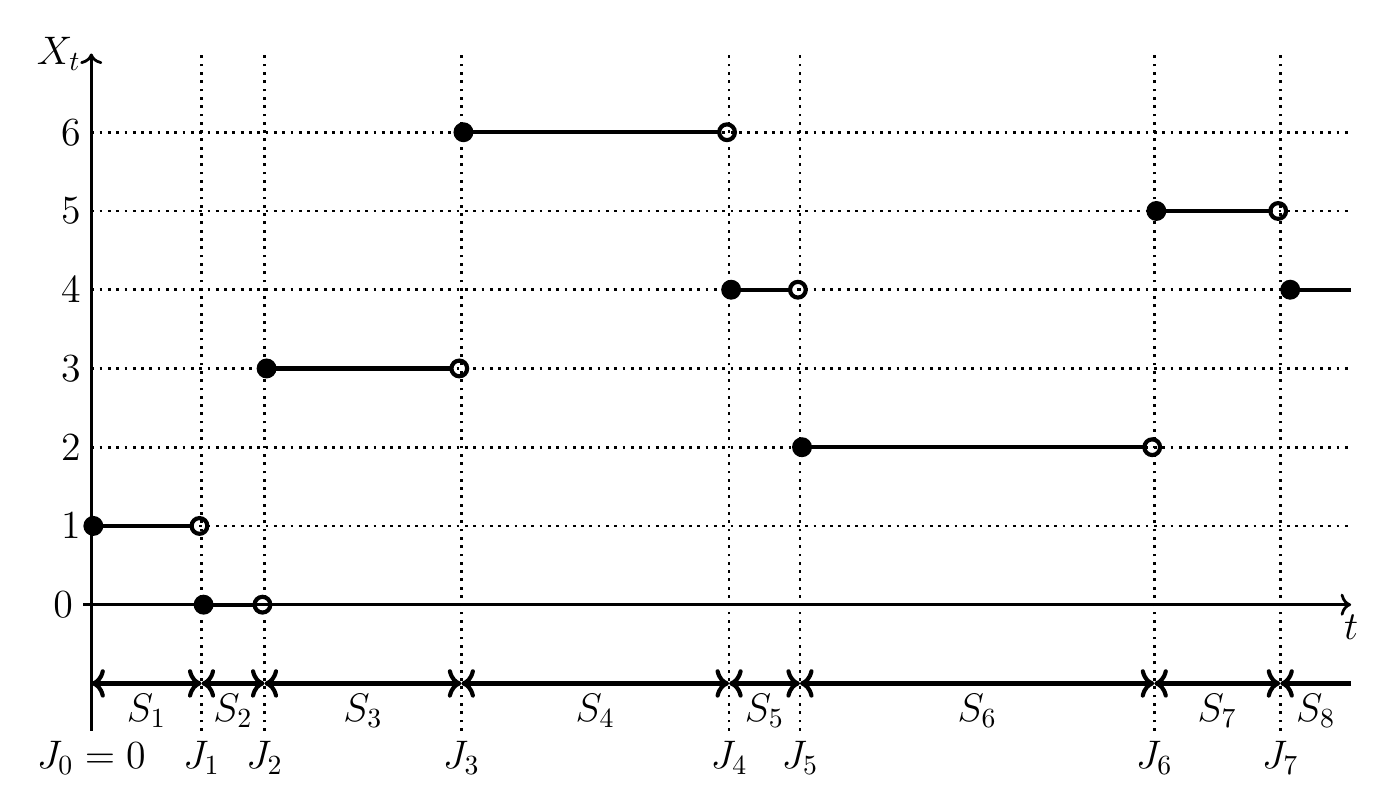
\begin{tikzpicture}

		\draw[very thin,color=gray];
		\draw[->, line width=1] (-0.1,0) node[left] {\Large$0$} -- (16,0) node[below] {\Large$t$}; 
		\draw[->, line width=1] (0,-1.6) node[below] {\Large$J_0=0$} -- (0,7) node[left] {\Large$X_t$};
		
		% make the horizontal dotted lines
		\draw[dotted, line width=1] (-0.0,1) node[left] {\Large$1$} -- (16,1);
		\draw[dotted, line width=1] (-0.0,2) node[left] {\Large$2$} -- (16,2);
		\draw[dotted, line width=1] (-0.0,3) node[left] {\Large$3$} -- (16,3);
		\draw[dotted, line width=1] (-0.0,4) node[left] {\Large$4$} -- (16,4);
		\draw[dotted, line width=1] (-0.0,5) node[left] {\Large$5$} -- (16,5);
		\draw[dotted, line width=1] (-0.0,6) node[left] {\Large$6$} -- (16,6);
		 
		% make the 7 time jumps, J0, J1, ..., J6
		\draw[dotted, line width=1] (1.4,-1.6) node[below] {\Large$J_1$} -- (1.4,7);
		\draw[dotted, line width=1] (2.2,-1.6) node[below] {\Large$J_2$} -- (2.2,7);
		\draw[dotted, line width=1] (4.7,-1.6) node[below] {\Large$J_3$} -- (4.7,7);
		\draw[dotted, line width=1] (8.1,-1.6) node[below] {\Large$J_4$} -- (8.1,7);
		\draw[dotted, line width=1] (9.0,-1.6) node[below] {\Large$J_5$} -- (9.0,7);
		\draw[dotted, line width=1] (13.5,-1.6) node[below] {\Large$J_6$} -- (13.5,7);
		\draw[dotted, line width=1] (15.1,-1.6) node[below] {\Large$J_7$} -- (15.1,7);
		
		% make the Xt value arrows
		\draw[line width=1.5, -Circle] (16.0,4) -- (15.1, 4);
		\draw[line width=1.5, Circle-{Circle[open]}, postaction=decorate] (13.4, 5) -- (15.2,5);
		\draw[line width=1.5, Circle-{Circle[open]}, postaction=decorate] (8.9, 2) -- (13.6,2);
		\draw[line width=1.5, Circle-{Circle[open]}, postaction=decorate] (8.0, 4) -- (9.1,4);
		\draw[line width=1.5, Circle-{Circle[open]}, postaction=decorate] (4.6, 6) -- (8.2,6);
		\draw[line width=1.5, Circle-{Circle[open]}, postaction=decorate] (2.1, 3) -- (4.8,3);
		\draw[line width=1.5, Circle-{Circle[open]}, postaction=decorate] (1.3, 0) -- (2.3,0);
		\draw[line width=1.5, Circle-{Circle[open]}, postaction=decorate] (-0.1, 1) -- (1.5,1);
		
		% make the holding time arrows
		\draw[line width=1.5, <-, postaction=decorate] (15.1, -1) -- (16.0,-1) node [midway, below] {\Large$S_8$};
		\draw[line width=1.5, <->, postaction=decorate] (13.5, -1) -- (15.1,-1) node [midway, below] {\Large$S_7$};
		\draw[line width=1.5, <->, postaction=decorate] (9.0, -1) -- (13.5,-1) node [midway, below] {\Large$S_6$};
		\draw[line width=1.5, <->, postaction=decorate] (8.1, -1) -- (9.0,-1) node [midway, below] {\Large$S_5$};
		\draw[line width=1.5, <->, postaction=decorate] (4.7, -1) -- (8.1,-1) node [midway, below] {\Large$S_4$};
		\draw[line width=1.5, <->, postaction=decorate] (2.2, -1) -- (4.7,-1) node [midway, below] {\Large$S_3$};
		\draw[line width=1.5, <->, postaction=decorate] (1.4, -1) -- (2.2,-1) node [midway, below] {\Large$S_2$};
		\draw[line width=1.5, <->, postaction=decorate] (0.0, -1) -- (1.4,-1) node [midway, below] {\Large$S_1$};

		
	\end{tikzpicture}
\end{document}